%\documentclass[justified, marginals=raggedouter]{tufte-handout}
\documentclass[justified, marginals=justified]{tufte-handout}

% Adding a few custom packages
\usepackage{tcolorbox}
\usepackage{lipsum}

% The default minimumo amount of space between \marginnotes is 10 pt.
\setlength\marginparpush{1cm}

\title{6.864 Advanced Natural Language Processing\thanks{Instructors: Prof. Regina Barzilay, and Prof. Tommi Jaakkola.\\ TAs: Franck Dernoncourt, Karthik Rajagopal Narasimhan, Tianheng Wang. \\ Scribes: Brandon Carter, Sarah Vente.}}

\author[Lecture 1: Introduction]{Lecture 1: Introduction}

\date{9 September 2015} % without \date command, current date is supplied

%\geometry{showframe} % display margins for debugging page layout

\usepackage{graphicx} % allow embedded images
  \setkeys{Gin}{width=\linewidth,totalheight=\textheight,keepaspectratio}
  \graphicspath{{graphics/}} % set of paths to search for images
\usepackage{amsmath}  % extended mathematics
\usepackage{booktabs} % book-quality tables
\usepackage{units}    % non-stacked fractions and better unit spacing
\usepackage{multicol} % multiple column layout facilities
\usepackage{lipsum}   % filler text
\usepackage{fancyvrb} % extended verbatim environments
  \fvset{fontsize=\normalsize}% default font size for fancy-verbatim environments

% Standardize command font styles and environments
\newcommand{\doccmd}[1]{\texttt{\textbackslash#1}}% command name -- adds backslash automatically
\newcommand{\docopt}[1]{\ensuremath{\langle}\textrm{\textit{#1}}\ensuremath{\rangle}}% optional command argument
\newcommand{\docarg}[1]{\textrm{\textit{#1}}}% (required) command argument
\newcommand{\docenv}[1]{\textsf{#1}}% environment name
\newcommand{\docpkg}[1]{\texttt{#1}}% package name
\newcommand{\doccls}[1]{\texttt{#1}}% document class name
\newcommand{\docclsopt}[1]{\texttt{#1}}% document class option name
\newenvironment{docspec}{\begin{quote}\noindent}{\end{quote}}% command specification environment

\begin{document}

\maketitle% this prints the handout title, author, and date

This first lecture introduces Natural Language Processing (NLP). It presents the core concepts of NLP, some of its main applications as well as challenges, a succinct history of the field, and machine learning approaches.

\section{Definition of Natural Language Processing (NLP)}\label{sec:what-is-nlp}

TODO


\section{Applications}\label{sec:nlp-applications}
TODO 


\section{Challenges}\label{sec:nlp-challenges}
TODO


\section{History}\label{sec:nlp-history}

TODO

\section{Applying Machine Learning Methods}\label{sec:applying-machine-learning-methods}

\subsection{The Determiner Placement Task}\label{sec:determiner-placement-task}

The determiner placement task is defined as follows: given a text with no determiner, add any missing determiner to the text. For example, the given text could be ``\textit{Scientists in United States have found way of turning lazy monkeys into workaholics using gene therapy.}''. To simplify the task, assume that we only consider one sort of determiner, the definite article \textit{the}. The decision is therefore binary, viz. whether \textit{the} should precede a given noun in a given text.

%To simplify the task, assume we only consider determiners that are articles, viz. the definite article \textit{the} and the indefinite articles \textit{a} and \textit{an}.

%\begin{tcolorbox}[colback=green!5,colframe=green!40!black,title=Determiner Placement example]
%\begin{tcolorbox}[colback=green!5,colframe=green!40!black]
%Scientists in United States have found way of turning lazy monkeys into
%workaholics using gene therapy. Usually monkeys work hard only when
%they know reward is coming, but animals given this treatment did their
%best all time.
%\end{tcolorbox}

%For a native English speaker, performing this task is usually easy. However, there exist many grammar rules specifying determiner placements, as well as numerous exceptions. While the determiner placement mostly result from the countability of the noun (i.e. whether it is countable or uncountable), the uniqueness of reference – Information value (given, new) – Number (singular, plural)


% About the the uniqueness of the reference: https://books.google.com/books?id=ZN9eAgAAQBAJ&pg=PA148&lpg=PA148&dq=%22uniqueness+of+the+reference%22&source=bl&ots=ukoGCJeJIf&sig=L55rz7Qal3ylO1861CGMHk6isBE&hl=en&sa=X&ved=0CCgQ6AEwAmoVChMIgdftxLCByAIVSjk-Ch2dNgVW#v=onepage&q=%22uniqueness%20of%20the%20reference%22&f=false
For a native English speaker, performing this task is usually easy. However, there exist many grammar rules specifying determiner placement, based on linguistic knowledge such as the countability of the noun (i.e. whether it is countable or uncountable) or the plurality of the noun (i.e. whether it is singular or plural), as well as on world knowledge such as the uniqueness of reference (\textit{the current president of the US}) or the situational associativity between nouns (\textit{the score of the football game}). In addition to these generic grammar rules, there exist numerous exceptions: for instance, while the definite article is required in newspaper titles (e.g. \textit{The Times}), it shall not be used for names of magazines and journals (e.g. \textit{Time}). %Moreover, ambiguities might arise from the world knowledge.

%in addition to placing a determiner, there are other considerations such as noun plurality, in which the determiners ``this'' and ``that'' also have respective plural forms ``these'' and ``those.'' Deciding plurality adds an additional layer of complexity in determiner placement. 

%Furthermore, there are many ambiguous cases, such as in the sentence ``Apples are fruits'' because a complete noun phrase is formed without any determiner. Determiners can also be used in certain combinations, like ``all the chairs.''
Given the amount of rules and exceptions involved in determiner placement, it would be tremendously difficult to manually encode all of this information: a symbolic system for the determiner placement task would subsequently be difficult to successfully construct.

\subsection{Determiner Placement as a Supervised Classification Task}\label{sec:determiner-prediction-as-classification}

% by casting it into a classification task.
As an alternative to the symbolic approach, one could adopt a statistical approach to the determiner placement task by casting it as a supervised classification task. %To further simplify the task, assume the classifier's goal is to predict whether \textit{the} should precede a given noun in a given text. In other words, the classifier prediction is binary.
%The classifier's goal is to predict whether \textit{the}, \textit{a}, or \textit{an} should precede a given noun in a given text.

\medskip

A basic classifier could be trained as follows:

\begin{enumerate}
\item Gather a large collection of texts (e.g. a set of newspaper articles) and split it into a training set and a test set.
\item For each noun in the training set, compute the probability it follows a certain determiner, i.e. $p(\text{determiner}| \text{noun)} = \frac{\text{count(determiner, noun)}}{count(noun)} $.
\item Given a text from the test set where determiners have been removed, for each noun in the text, select the determiner with the highest probability as estimated in the previous step.
\end{enumerate}

The quality of the predictions made by this classifier is not outstanding, but still surprisingly high for such a simple method: using the first 21 sections of the Wall Street Journal (WSJ) corpus as the training set, and the 23rd section as the test set, the prediction accuracy is 71.5\%. This result can be used as a baseline for more elaborate classifiers.

\medskip

The typical steps to train a classifier in a supervised fashion are as follows:

%\marginnote{The usual steps to train a classifier: data collection, data labeling, feature extraction, training, testing.}

\begin{enumerate}
\item \textit{Data collection}: Gather a large collection of texts, and split it into a training set and a test set. Because one can easily get a training set of sample sentences in English with correct determiner placement, no addition work is needed to obtain the labels: we assign a label $-1$ or $+1$ to each noun ($+1$ if the noun is preceded by a determiner, $-1$ if not).
\item \textit{Feature extraction}: For each noun in the training and test sets, extract some features. E.g. whether the noun plural is plural ($0$ if no, $1$ if yes), whether it is its first appearance in the text ($0$ if no, $1$ if yes), and so on. We therefore obtain one feature vector for each noun. Figure~\ref{fig:feature-extraction} illustrates the process of feature extraction.
\begin{marginfigure}[-3cm]%
\centering
  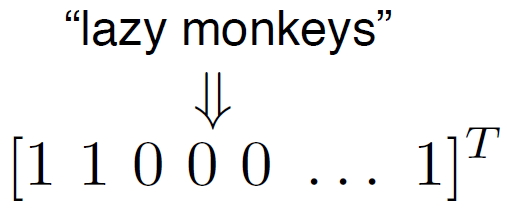
\includegraphics[width=3cm]{feature-extraction.png}
  \caption{\textbf{Feature extraction} is the process of converting a text to a feature vector, before feeding it to a classifier. If there are $n$ binary features, then the feature vector will be of dimension $n$.}
  \label{fig:feature-extraction}
\end{marginfigure}
\item \textit{Training}: Train a classifier using the extracted features as well as the labels. The training step is used to find the optimal feature weight vector to improve the final prediction. Figure~\ref{fig:linear-separator-learning} shows a decision boundary (in simplified two-dimensional space) based on the feature vectors and weight vectors.
\item \textit{Testing}: Assess the classifier's prediction quality on the test set. Using this machine learning approach, one can reach an accuracy above 86\%.
\end{enumerate}



\begin{marginfigure}
  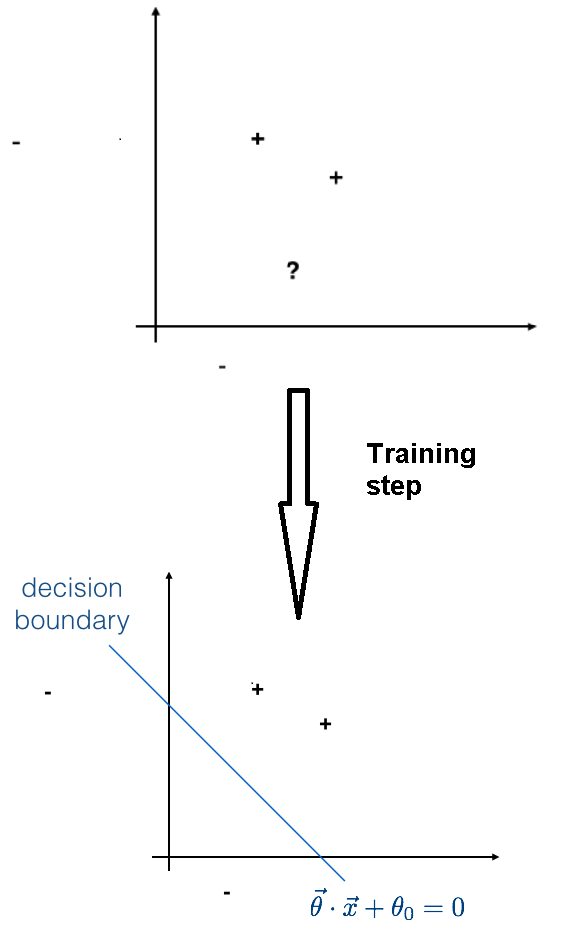
\includegraphics[width=\linewidth]{linear-separator-learning.png}
  \caption{Learning the \textbf{decision boundary} based on the feature vectors and weight vectors. In this example (in simplified two-dimensional space), there are two positive points (with $+$ labels), and two negative points (with $-$ labels). The decision boundary correctly separates all of the training points.}
  \label{fig:linear-separator-learning}
\end{marginfigure}


Table~\ref{tab:samples-for-classifiers} shows pairs of features and label that result from step 1 and~2. To train the classifier in step 3 using these features and labels, there exist many classification algorithms such as the perceptron algorithm. The perceptron algorithm iterates through the training examples and finds an optimal decision boundary to separate as many of the training points as possible: it places the decision boundary so that it optimizes the number of training points that are classified correctly, as shown in Figure \ref{fig:linear-separator-learning}. 

Once the decision boundary is placed, one can plot any new vector into this space and determine on which side of the decision boundary it is located. A noun whose vector falls on the $+1$ side is assigned a $+1$ label, while a noun whose vector fall on the other side of the boundary is assigned a $-1$ label. This classification procedure therefore utilizes the training examples with known determiner placement to classify the unlabeled examples.


\begin{table}[h]
\begin{center}
\begin{tabular}{lccccc}
\toprule
 & \multicolumn{3}{c}{Features}  \\
\cmidrule(l){2-4} 
Noun & plural? & 1st appearance? & unigram & label\\
\midrule
Scientists & 1 & 1 & 00100 & null \\
United States & 1 & 1 & 00010 & the\\
lazy monkeys & 1 & 1 & 00001 & the\\
gene therapy & 0 & 1 & 01000 & null\\
\bottomrule
\end{tabular}
\end{center}
\caption{Example of feature values and labels given to the classifier during the training phase. This table results from data collection, labeling and feature extraction. The feature values for the unigram feature present in this table are much smaller than it is in reality: unigram feature values are one-hot vectors of dimension $|V|$, where $V$ is the dictionary.}
\label{tab:samples-for-classifiers}
\end{table}

\begin{marginfigure}[4cm]
\centering
  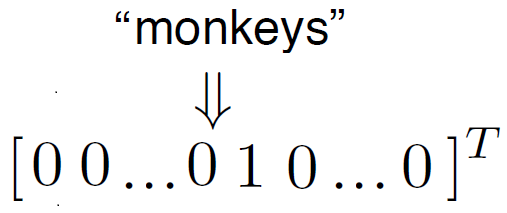
\includegraphics[width=3cm]{feature-extraction-unigram.png}
  \caption{Extracting an unigram feature is the process of converting a word to a one-hot vector, which will be used as a feature.}
  \label{fig:feature-extraction-unigram}
\end{marginfigure}

%Choosing the right features, aka. feature engineering, is of paramount importance.
One of the most common features in NLP is word \textit{n-grams}, or simply n-grams. A word n-gram is a sequence of $n$ words. A unigram designates a 1-gram, a bigram is a 2-gram, and a trigram is a 3-gram. n-gram of larger sizes are less often used.  An n-gram feature value is encoded as a \textit{one-hot vector}, i.e. a vector in which all elements are 0 except one element that is 1. For example, $[0, 0, 0, 1, 0]$ is a one-hot vector. If the vocabulary is of size $|V|$, then there are $|V|$ possible unigrams, $|V|^2$ possible bigrams, and $|V|^3$ possible trigrams. This means that the unigram feature value will be a one-hot vector of dimension $|V|$, the bigram feature value will be a one-hot vector of dimension $|V|^2$, and the trigram feature value will be a one-hot vector of dimension $|V|^3$. Despite its simplicity, using n-gram as a feature often yields high performances: if the unigram feature is added to the classifier in the determiner placement task (i.e. the unigram feature is extracted from the noun, as shown in Figure~\ref{fig:feature-extraction-unigram}), it significantly improves the accuracy of the classifier. However, n-gram features are very sparse, since $|V|$ is typically very large, often over $10^4$.






\subsection{Limitations of Traditional Machine Learning Approaches}\label{sec:ml-limitations}

This traditional machine learning approach has several issues, the two main ones being the sparsity of the feature vectors and feature engineering:

%because the size of the vocabulary is generally very large, and therefore 

\begin{itemize}
\item \textit{Sparsity}: feature vectors are typically high-dimensional and sparse (i.e. most elements are $0$). Figure~\ref{fig:sparsity} illustrates that sparsity often results in many feature vectors not being seen when the training set is small. Figure~\ref{fig:sparsity2} shows the impact of sparsity on accuracy of parsers for different languages. 
\item \textit{Feature Engineering}: the second problem with using traditional machine learning approaches for classification is feature engineering. Early studies spent much time engineering features. Traditionally, features of compositional objects are manually-selected concatenations of atomic features, as Figure~\ref{fig:feature-engineering} illustrates. However, crafting these features by hand is difficult and time-consuming as they are combinatorial and the number of them is therefore extremely large.
\end{itemize}


\begin{figure}
  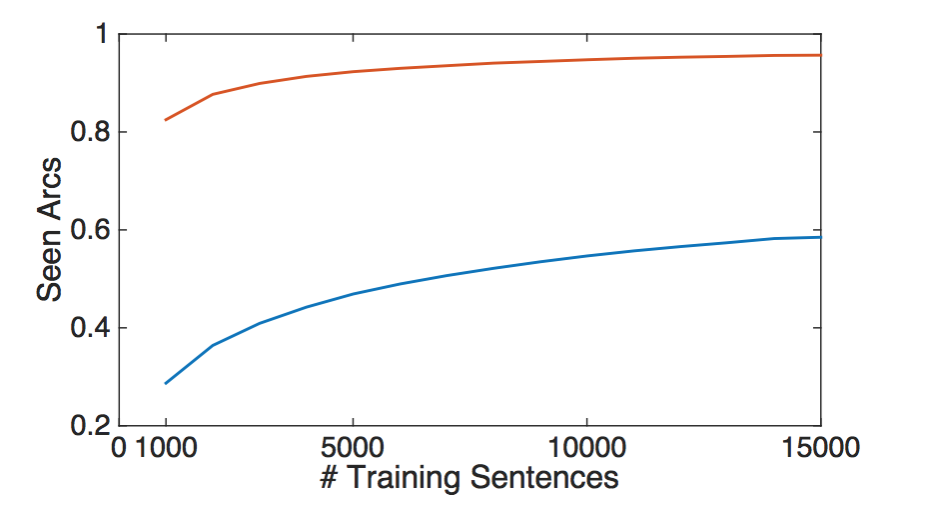
\includegraphics[width=\linewidth]{sparsity.png}
  \caption{In this graph, the red line indicates the portion of unigrams (single words) in the unseen tests that has already been seen in training. The first 1000 training sentences contain over 80\% of unigrams, and the first 10000 about 90\% of them. The blue line in the graph indicates the portion of bigrams (pairs of words) in the unseen samples that has already been seen in the training samples: this number is a lot lower than that for unigrams. Thus, if we consider bigrams for classification, it becomes difficult to be able to accurately classify unseen examples when the classifier has not seen the majority of bigrams during the training phase.} %  This is a problem of sparsity because of the massive number of possibilities of bigrams, since if our vocabulary is of size $|V|$, then there are $|V|^{2}$ possible bigrams, and $|V|$ is usually very large. 
  \label{fig:sparsity}
  \centering
  %\setfloatalignment{b}% forces caption to be bottom-aligned
%  \forceversofloat
\end{figure}
\vspace{55pt}
\begin{figure}
  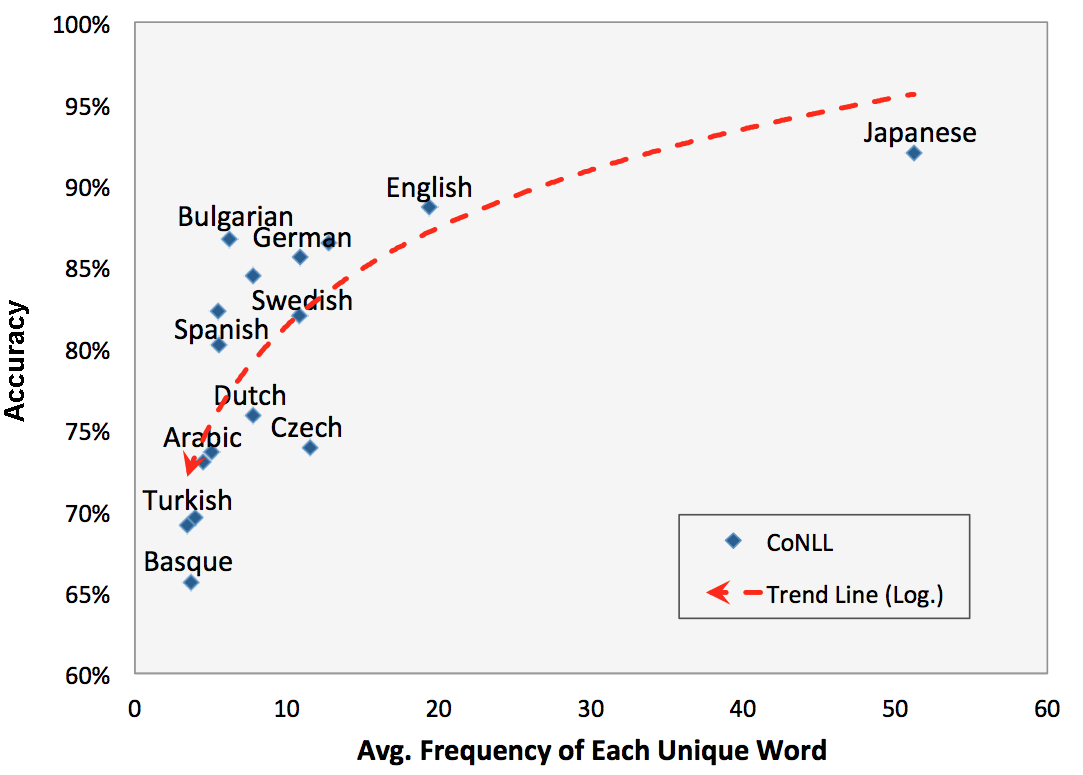
\includegraphics[width=\linewidth]{sparsity2.png}
  \caption{This graph shows the impact of sparsity on the accuracy of parsers for different languages. Japanese and English have the highest accuracies, and a good predictor of the parser accuracy is the average frequency of each unique word. This means that the parser has a much greater accuracy when it can be trained on larger subsets of the words that will appear in the test set.}
  \label{fig:sparsity2}
  \centering
  %\setfloatalignment{b}% forces caption to be bottom-aligned
%  \forceversofloat
\end{figure}


\begin{figure}
  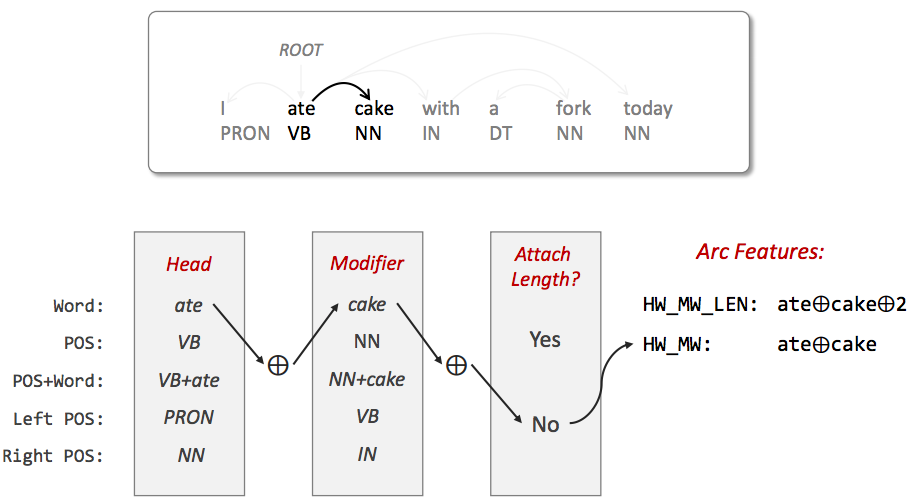
\includegraphics[width=\linewidth]{feature-engineering.png}
  \caption{Selecting feature representation. Traditionally, features of compositional objects are manually-selected concatenations of atomic features.}
  \label{fig:feature-engineering}
  \centering
  %\setfloatalignment{b}% forces caption to be bottom-aligned
%  \forceversofloat
\end{figure}

\begin{marginfigure}[0.5cm]
  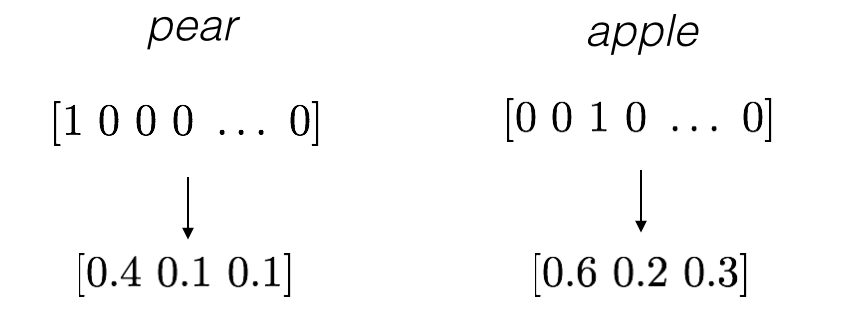
\includegraphics[width=\linewidth]{embeddings1.png}
  \caption{The words ``pear'' and ``apple'' are mapped from one-hot vectors to continuous, dense vectors of much lower dimension, where they are located close to each other.}
  \label{fig:embeddings1}
\end{marginfigure}

\subsection{Word Embeddings}\label{sec:word-embeddings}

Word embeddings are one solution to the sparsity problem. Embeddings are a set of machine learning techniques involving artificial neural networks that map discrete, one-hot vectors into low-dimensional continuous representations. They compress large sparse vectors into smaller, dense vectors, with semantically related words located close to each other in the word embedding space, as Figures~\ref{fig:embeddings1} and \ref{fig:embeddings2} show. The word embedding space also contains interesting linear substructures, as Figure~\ref{fig:word-embeddings-linear-substructures} illustrates: word embeddings are very powerful as they can capture some semantic relations between words.



\begin{figure}
  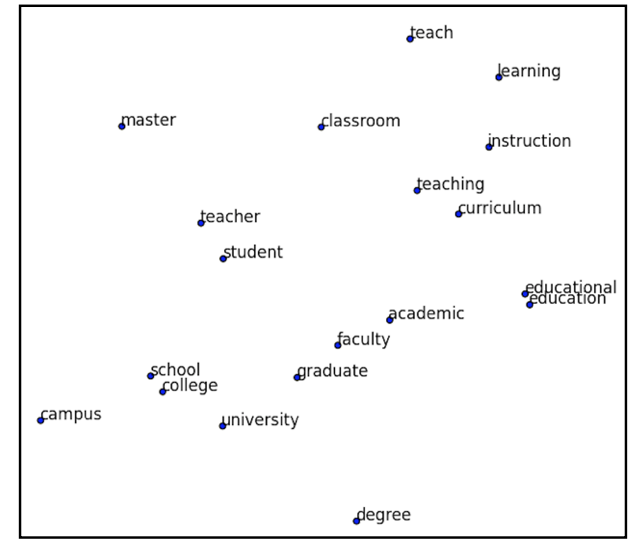
\includegraphics[width=1.0\linewidth]{embeddings2.png}
  \centering
  \caption{t-SNE visualization of word embeddings (t-SNE stands for t-Distributed Stochastic Neighbor Embedding). This plot illustrates a projection of embedded vectors into 2-D space. Semantically close words such as ``school'' and ``college'' are mapped closely to one another in the word embedding space, whereas they would appear unrelated when encoded as one-hot vectors. Source: \url{http://nlp.yvespeirsman.be}}
  \label{fig:embeddings2}
\end{figure}

\begin{figure}
  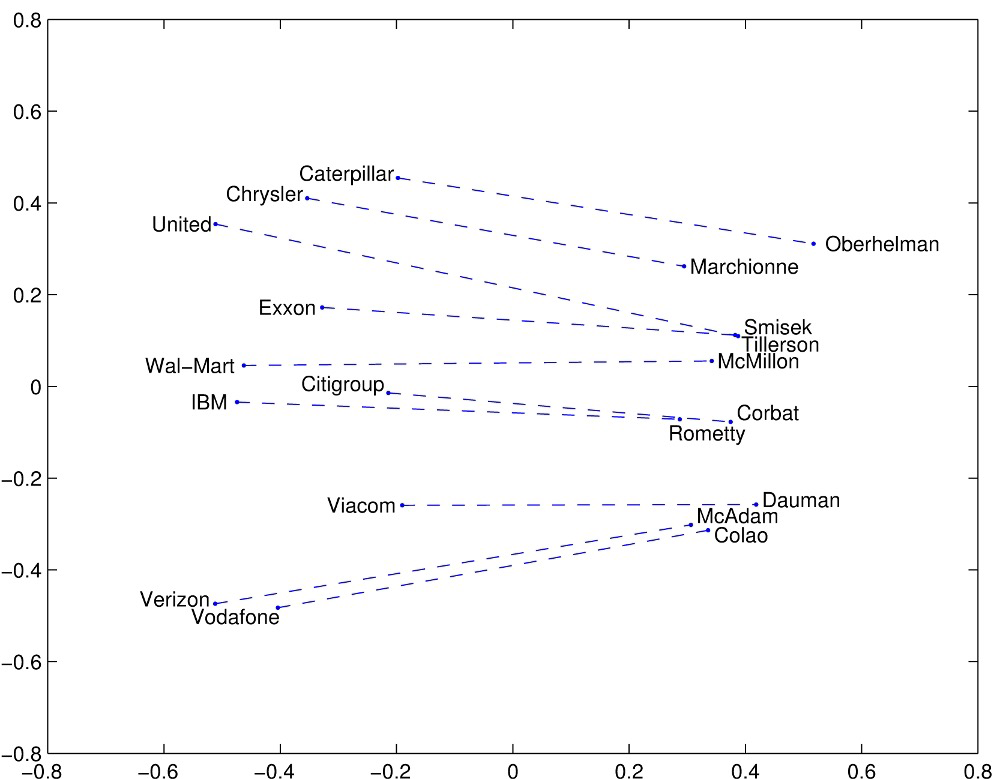
\includegraphics[width=1.0\linewidth]{word-embeddings-linear-substructures.png}
  \caption{Linear substructures in word embeddings. In this example, if we take the embedding corresponding to the CEO of one company, subtract that company, and add another company, we will arrive at the CEO of the other company. Source: \url{http://nlp.stanford.edu/projects/glove}}
  \label{fig:word-embeddings-linear-substructures}
\end{figure}


\begin{marginfigure}
  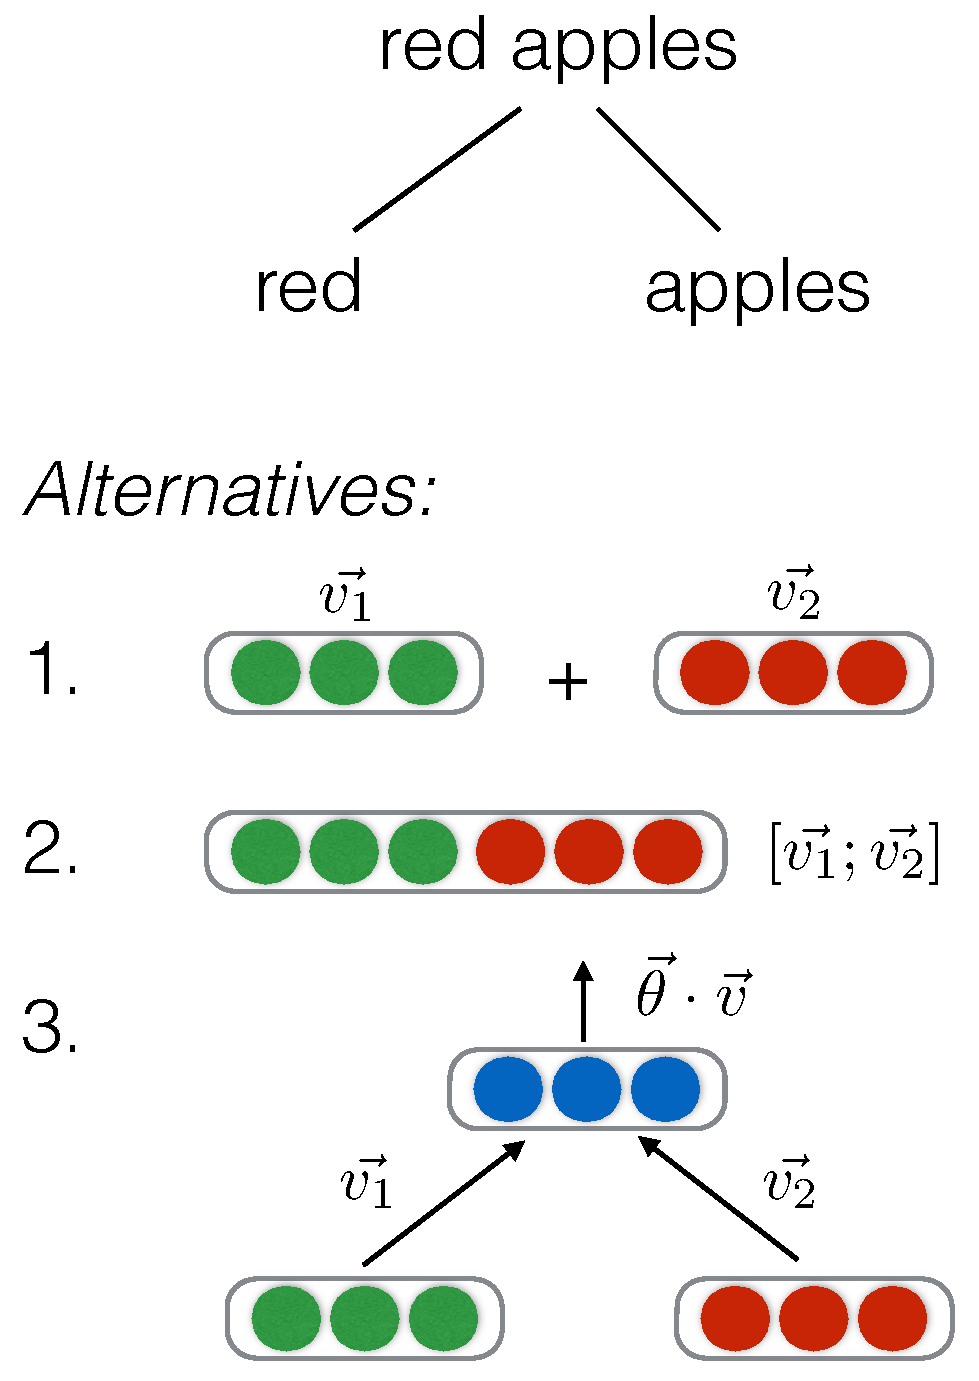
\includegraphics[width=\linewidth]{learning-feature-representations.pdf}
  \caption{Three strategies amongst others to combine word embeddings.}
  \label{fig:learning-feature-representations}
\end{marginfigure}


\medskip


Word embeddings are also one solution to the problem of feature engineering. Suppose we are trying to find a feature representation for the phrase ``red apples.'' We could start with the word embedding vector for ``red'' and the word embedding vector for ``apples''. Then, we could add them, concatenate them, or combine them otherwise, as Figure~\ref{fig:learning-feature-representations} illustrates. Traditionally, we would just engineer features and use them for the main problem that requires these features. Using word embeddings, one can learn them jointly with the learning problem, for example by adding a hidden layer in learning problem, which allows us to learn compositional meaning in the vector space, optimize the feature representation, and then carry it forward to the final NLP task.\medskip

In general, one can tackle NLP tasks using traditional machine learning approaches, or newer techniques based on artificial neural networks. This course will cover both approaches. 

%\bibliography{lecture01}
%\bibliographystyle{plainnat}



\end{document}
